 %!TeX root = PHYS42 Lecture Notes.tex
\documentclass{article}
\usepackage[dvipsnames, svgnames, x11names]{xcolor}
\usepackage{tikz}
\usepackage{pgfplots}
\usepackage{pgfplotstable}
\usepackage{setspace}
\usepackage{units}
\usepackage{booktabs}
\usepackage{graphicx}
\usepackage{amsfonts}
\usepackage{circuitikz}
\usepackage{multirow}
\usepackage{amsopn}
\usepackage{bbding}
\usepackage{amsmath}
\usepackage{hyperref}
\usepackage{cancel}
\usepackage{gensymb}
\usepackage[margin = 1.2in]{geometry}

\newcommand{\midlabelline}[3]{
   \node (midlabel) at ($ (#1)!.5!(#2) $) {#3};
   \draw[latex-] (#1) --  (midlabel);
   \draw[-latex] (midlabel) -- (#2);
}

\AtBeginEnvironment{document}{\everymath{\displaystyle}}
\title{MATH 2 Lecture Notes}
\date{Tuesday, 14 January, 2025}
\author{Tejas Patel}
\begin{document}
\maketitle
\tableofcontents
\pagebreak
\section{Chapter 1}
\subsection{Terminology}
\textbf{Definition} A differential equation is an equation containing the derivatives or differentials 
of one or more dependent variables, with respect to one or more independent variables.\\
\textbf{$\cdot$} An Ordinary Differential Equation (ODE) involves only ordinary derivatives\\
\textbf{$\cdot$} A Partial Differential Equation (PDE) involves partial derivatives.\\
\textbf{Definition} The order of a DE is the order of the highest-order derivative that appears in the DE
\textbf{Notation} $F(x,y,\frac{dy}{dx}, \frac{d^2y}{dx^2})$\\
\textbf{Definition} A linear DE is any DE that can be written in form:\\
${\displaystyle a_{0}(x)y+a_{1}(x)y'+a_{2}(x)y''\cdots +a_{n}(x)y^{(n)}=b(x)}$\\
For a DE to be linear:
\begin{enumerate}
    \item Y and all of its derivatives much be of the 1st degree
    \item Any term that does not include y or any of its derivatives must be a function of x
\end{enumerate}
\subsection{Some Mathematical Models}
\subsubsection*{I. Free-falling body}
Goal: Find s(t). 
\\Set up a differential equation in S, model it, then solve
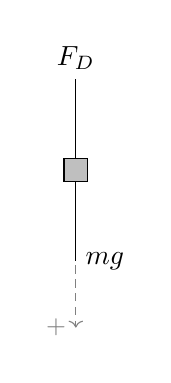
\begin{tikzpicture}[
    force/.style={>=latex,draw=blue,fill=blue},
    axis/.style={densely dashed,gray,font=\small},
    M/.style={rectangle,draw,fill=lightgray,minimum size=0.5cm,thin},
    m/.style={rectangle,draw=black,fill=lightgray,minimum size=0.3cm,thin},
    plane/.style={draw=black,fill=blue!10},
    string/.style={draw=red, thick},
    pulley/.style={thick},
]
\matrix[column sep=1cm] {
    \node[m] (m) {};

    \draw[axis,->] (m) -- ++(0,-2) node[left] {$+$};
    {[force,->]
    \draw (m.north) -- ++(0,1) node[above] {$F_D$};
        \draw (m.south) -- ++(0,-1) node[right] {$mg$};
    }
\\
};
\end{tikzpicture}\\
$ma=mg\\\frac{d^2s}{dt^2}=g\\v=\frac{ds}{dt}, g=\frac{dv}{dt}$\\
What if there is air resistance. Assume force scales linear with velocity
\\$\frac{dv}{dt}=g-\frac{kv}{m} \rightarrow \frac{dv}{dt}=g-\frac{k}{m}\cdot \frac{ds}{dt}$
\subsubsection*{II: Series Circuit}
\begin{circuitikz}
    \draw[line width=0.8]
     (2,7) to [sinusoidal voltage source, l_=$V_S$, i=$I$] (2,1)
     (2,7) to [resistor, l_=$R$] ++(6,0) to [inductor, l_=$L$] ++(0,-6) to [capacitor, l_=$C$] +(-6,0) ;
    \midlabelline{2,8}{8,8}{$V_R$}
    \midlabelline{9,7}{9,1}{$V_L$}
    \midlabelline{2,0}{8,0}{$V_C$}
\end{circuitikz}

Voltage drops:\\ $
V=L \frac{dI}{dt}, V=L \frac{d^2q}{dt^2}\\
V=IR, V= R \frac{dq}{dt}\\
V=\frac{q}{C}\\
E(t) = L \frac{d^2q}{dt^2}+ R \frac{dq}{dt} + \frac{q}{C}
$
\subsubsection*{III: Population Growth}
$P=P(t) =$ population at time t — use exponential model \\
$\frac{dp}{dt} \propto P \rightarrow \frac{dp}{dt} = kP \rightarrow = Ce^{kt}$ where C is the initial population
\subsubsection*{IV: Population Growth with Finite Capacity}
"Carrying Capacity" = N — uses the logistic growth model\\
$\frac{dp}{dt} \propto $ both P and amount to carrying capacity (N-P)\\
$\frac{dp}{dt}=kP(N-P)$
\subsubsection*{V: Chemical Reaction}
$A+B\rightarrow C$ Concentrations of A and B decreases by amount of C formed \\ 
Can we write DE governing the concentration of C x(t)? \\ 
The rate at which the reaaction takes place $\propto$ Product of the remaining concentrations of A and B
\\ $\alpha$ initial concentration of A
\\ $\beta$ initial concentration of B
\\ $\frac{dx}{dt} = k(\alpha - x)(\beta - x)$
\section{First-Order Differential Equations}
\subsection{Preliminary Theory}
Example DE: $y'=3y \Rightarrow \boxed{y=Ce^{3x}}$ the general solution where C is an arbitrary constant
\\[0.05in]Add initial condition $y(0) = 5$ plug in x=0 to $5=Ce^{3*0}, 5=C*1, C=5 \Leftarrow$ Initial Value Problem
\\$y=5e^{3x}$ is the general solution for the Initial Value Problem\\\subsubsection{\textbf{Theorem}}
$f(x) = \begin{cases}
    \frac{dy}{dx} = f(x,y) & \text{Differential Equation}\\
    y(x_0) = y_0  & \text{Initial Condition}
    \end{cases}$\\ Let R be a rectangular region in the xy-plane defined by $a\leq x \leq b, c \leq y \leq d $, that contains the point $(x_0, y_0)$ in its interior. \\[0.1in] If f(x,y) and $\frac{\partial f}{\partial y}$ are continuous on $R$, then there exists an interval I centered at $x_o$, and on this interval $I$ there exists a unique solution $y(x)$ for this IVP\\
\subsubsection{\textbf{Key Questions:}}Does every IVP have at least one solution?\\ If an IVP has a solution is it the only solution?

\textbf{Meaning of a solution existing "on an Interval"}
The initial value problem
\\$\begin{cases}
    \frac{dy}{dx} =1+y^2
    \\ y(0)=0
\end{cases}$ has a unique solution. In fact, we can easily verify that $y=\tan x$ satisfies this IVP
\\ However note that there are some inervals on which $y=\tan x$ cannot be a solution for this IVP, such as (-2,2),
where the function is discontinuous at $\pm \frac{\pi}{2}$ but can be used for (-1,1) since it is continuous at all points within the interval
\subsection{Separable Variables (Separable Equations)}
\subsubsection{\textbf{Definition: }}A differential equation that can be written in the form $\frac{dy}{dx}= \frac{g(x)}{h(y)}$ is said to be separable (or have separable variables).
\\\textbf{Example: } $\frac{dy}{dx}= \frac{g(x)}{h(y)} \\[0.05in]h(y) dy = g(x) dx \\[0.05in] \int{h(y)}{dy} = \int g(x) dx$ 
\\\textbf{Example: } $dx+e^{3x}dy=0$ \\ $e^{3x} dy = -dx$ \\ $dy=-\frac{dx}{e^{3x}}\rightarrow dy=-{e^{-3x}}{dx} \rightarrow \int dy=\int -{e^{-3x}}{dx} \rightarrow y=\frac{1}{3}e^{-3x}+C$ where C is an arbitrary constant
\subsubsection{Substitution} $\frac{dy}{dx} = F(ax+bc+c)$ where $b\neq 0$ use the substitution: $u=ax+by+c \Rightarrow \frac{du}{dx} = a+b\frac{dy}{dx} = \frac{1}{b}\left[\frac{du}{dx}-a\right]$
\\Example: $\frac{dy}{dx} = \tan^2(x+y)$ let $u=x+y \rightarrow \frac{dy}{dx}=\frac{du}{dx}-1 \rightarrow \frac{du}{dx}-1=\tan^2 u \rightarrow \frac{du}{dx} = \sec ^2 u \\ \int \cos^2 u \; du = \int dx \\ 2(x+y)+\sin2(x+y) = 4x+C \rightarrow 2y-2x+\sin2(x+y)$
\\ \textbf{Solve:}
$\frac{dy}{dx} = (y+3)^2$ By inspection $y=-3$ is a solution. This is the only solution because $f(x,y)=(x+3)^2$ is continuous on $\mathbb{R}^2$ and $\frac{\partial f}{\partial x}$ is continuous on$ \mathbb{R}$ so it is the only solution
Why solving by separation is not possible
$\int (y+3)^-2 dy=\int dx \rightarrow (y+3)^-2/-1=x+C_1 \rightarrow \frac{1}{y+3}=-x-C_1 \rightarrow y+3 = \frac{1}{c-x} \rightarrow y=-3+\frac{1}{c-x}
\\y(0)=-3\rightarrow 0=\frac{1}{c}$ where there is no real c that solves that equation, making this not possible
\subsection{Homogeneous Equations} 
\textbf{What do we do if the DE is not separable?}
\subsubsection{Definition} A function $f(x,y)$ is said to be \textbf{homogeneous of degree} $n$ if, for $x, y,$ and$ t $where $f(x,y)$ and $f(tx,ty)$ are defined: \\$$f(tx,ty)=t^nf(x,y)$$
\subsubsection{Example} Determine wheteher each function is homogeneous: \\
a: $ f(x,y)=x^3-7x^2y+4y^3 \rightarrow f(tx,ty)=(tx^3)-7(tx)^2(ty)+4(ty)^3\\t^3x^3-7t^3x^2y+4t^3y^3\\t^3(x^3-7x^2y-4y^3)=t^3f(x,y)$
\\How to tell quickly wheteher $f(x,y)$ is homogeneous:
\\Each term must have the same combined degree
\\Example: $x^3-7x^2y+4y^3$ is D3, $x^2+y^2-4x$ is not, $\sqrt{x^5+4y^5}$ is with D 2.5, $\frac{3y}{x}-2$ is D0
\subsubsection{Differential Equation form}
$M(x,y)dx+N(x,y)dy=0$ is called a homogeneous differential equation if the functions $M$ and $N$ are both homogeneous of the same degree
\\If $f(x,y)$ is homogeneous of degree $n$ then $f(x,y)$ can be written as:
\\$f(x,y)=f\left(x\times 1, x \times \frac{y}{x}\right)=x^nf\left(1, \frac{y}{x}\right)$
\\or $f(x,y)=y^nf\left(\frac{x}{y},1\right)$
\subsubsection{Substitution} To solve a homogeneous DE make the substitution: $y=ux \;\; (u=\frac{y}{x})$ or$ x=vy \; \; (v=\frac{x}{y})$
\subsubsection{Example}
$(y^2+xy)dx+x^2dy=0 \rightarrow y=ux \rightarrow dy=(udx+xdu) \\ (u^2x^2+ux^2)dx+x^2(udx+xdu)=0\\u^2x^2dx+ux^2dx+ux^2dx+x^3du=0 \\ ux^2(u+2)dx+x^3du=0\\\int \frac{1}{u(u+2)}du=-\int \frac{1}{x}dx \\$ Partial Fraction Decomposition: $\frac{1}{u(u+2)}=\frac{A}{u}+\frac{B}{u+2} \rightarrow A=\frac{1}{2}, B=-\frac{1}{2}$ Back to solving \\ $\int \left[\frac{0.5}{u}-\frac{0.5}{u+2}\right]=-\int \frac{1}{x} dx \\ 0.5\ln|u|-1/2 \ln |u+2|=-\ln |x|+C_1 \\ \ln \left|\frac{u}{u+2}\right|=2C_1-2\ln|x| \\ \left|\frac{u}{u+2}\right|=e^{2C_1}\cdot e^{-2\ln|x|} = e^{2C_1}\cdot |x^{-2}| \Rightarrow \left|\frac{u}{u+2}\right| = \left|e^{2C_1}\cdot x^{-2}\right| \Rightarrow \left|\frac{u}{u+2} = \frac{C}{x^2}\right| \\ ux^2=X(u+2) \Rightarrow ux^2=Cu+2c \rightarrow ux^2-Cu=2C \\ u(x^2-c)=2C \Rightarrow u= \frac{2C}{x^2-C} \Rightarrow \frac{y}{x} = \frac{2Cx}{x^2-C}, \; x \neq 0$
\subsection{Exact Equations}
Recall from Math 1C: Let $F(x,y)=\langle 3x^2-7y, -7x+2y \rangle$
\begin{enumerate}
    \item If F a conservative vector field 
    \\i.e., Is there a function $f(x,y)$ such that $\nabla f$? Yes, -7=-7
    \item If F is indeed conservative, what is f? \\ $x^3-7xy+g(y)=f(x,y)\\-7x+2y, g'(y)=2y \\ f(x,y)=x^3-7xy+y^2+k$
\end{enumerate}
\subsubsection{Definition} A differential equation in the form $M(x,y)dx+N(x,y)dy=0$ where $M_y=N_x$, is called an exact differential equation.
\subsubsection{Solve the DE}
$(3x^2-7y)dx+(-7x+2y)dy=0$ \\Using 1C techniques it is $f(x,y)=x^3-2xy+y^2+k$
\\Set this f = c. $f(x,y)=x^3-2xy+y^2=c$ take k=0 in every problem
\\If the DE is not exact, sometimes we can make it exact by multiplying by magical quantity $\mu (x,y)$
\subsubsection{Example:} Solve the DE:
\\$(x+y)dx+xlnxdy=0$ using $\mu(x,y)=\frac{1}{x}$
\\$\left(\frac{x+y}{x}\right)dx+\ln|x|\;dy=0$ is now exact.
\\Solution: $f(x,y)=x+y\ln x=c$
\subsection{Linear Equations}
Recall: First Order Linear DE is a DE in the form $a_1(x)\frac{dy}{dx}+a_0(y)y=g(x),\qquad a_1(x)\neq 0$
\\Divide both sidex by $a_1(x) \Rightarrow \frac{dy}{dx}+\frac{a_0(x)}{a_1(x)}y=\frac{g(x)}{a_1(x)}$ where $P(x)=\frac{a_0(x)}{a_1(x)}$ and $f(x)=\frac{g(x)}{a_1(x)}$\\
\\$\frac{dy}{dx}+P(x)y=f(x)$ There is an integrating factor $\mu(x)$ that turns this DE into an exact DE
\\$dy+P(x)ydx=f(x)dx \rightarrow dy\left[P(x)y-f(x)\right] dx=0 
\\\mu(x)dy+\mu(x)\left[P(x)y-f(x)\right]dx=0 \rightarrow \mu '(x)=\mu(x)P(x) \\ \frac{d\mu}{dx}=\mu P
\rightarrow\int \frac{d\mu}{mu}=\int P(x)\rightarrow\ln\mu=\int P(x)\; dx
\\\mu(x)=e^{\int P(x)\; dx} \Rightarrow e^{\int P(x)\; dx} \frac{dy}{dx}+ e^{\int P(x)\; dx} P(x)y=e^{\int P(x)\; dx}f(x)
\\\frac{d}{dx}\left[e^{\int P(x)dx}y\right]=e^{\int P(x)dx}f(x) \rightarrow e^{\int P(x)dx}y=\int e^{\int P(x)dx}f(x)dx$
\boxed{y=e^{-\int P(x)dx}\int e^{\int P(x)dx}f(x) dx}
\subsubsection{Procedure to follow for every Linear DE}
\begin{enumerate}
    \item Rewrite the linear DE in the form $\frac{dy}{dx}+P(x)y=f(x)$
    \item Find the integrating factor $\mu(x)=e^{\int P(x)dx}$
    \item Multiply each side of the DE by $\mu(x)$
    \item Rewrite the left side as $\frac{d}{dx} \left[\mu(x)\cdot y\right]$
    \item Integrate both sides with respect to x and retreive an implicitly expressed solution
    \item Solve for y
\end{enumerate}
\subsection{What method to use to solve?}
First ask is it exact? $(M_y=M_x)$
\\Yes: Use the method in $\S$2.4
\\No: Is it linear? (in y or x)
\\Yes: Use the method in $\S$2.5
\\No: Is it separable?
\\Yes: $\S 2.2$
\\No: Homogeneous?
\\Yes: Use a substitution $\S 2.3$
\\No: Good luck. or use inspection\pagebreak
\section{Applications of First-Order Differential Equation}
\subsection{Orthogonal Trajectories}
$\cdot$ Consider the family of curves $y=cx^3$
Question: Which DE should be solved to get this family as its solutions?
\\Steps:
\begin{enumerate}
    \item Find $\frac{dy}{dx} =3cx^2$
    \item Eliminate c"
\end{enumerate} $y=cx^3 c=\frac{y}{x^3} \\ \frac{dy}{dx}=3\frac{y}{x^3}x^2 \rightarrow \frac{3y}{x}$

\textbf{$\cdot$} The two curves are orthogonal if their tangent lines are orthogonal at the point of intersection
\\i.e. The derivatives are the negative reciprocals of each other
\subsubsection{Example}
Show that $y=x^3$ and $x^2+3y^2=4$ are orthogonal at their points of intersection, (1,1) and (-1,-1)
\\ $y=x^3 \Rightarrow \frac{dy}{dx}=3x^2 \rightarrow =3$ at $x=1$ and 3 at $x=-1$
\\$2x+6y\frac{dy}{dx}=0 \rightarrow \frac{dy}{dx}=-\frac{x}{3y} = \frac{-1}{3}$ at both $x=1$ and $x=-1$ meaning it is orthogonal
\subsubsection{Definition} When all the curves of one family of curves intersect orthogonally all the curves of another family, then the families are said to be orthogonal trajectories of each other









\pagebreak
\section{Example Problems with Solutions}
\subsection{}
$\begin{cases}
    \frac{dy}{dx} = 2xy^\frac{2}{3}\\
    y(0) = 0  \\
\end{cases}$
$y=0$ and $y=\frac{x^6}{27}$ are solutions \\[0.05in]$\frac{dy}{dx} \frac{x^6}{27} = 2x \cdot \frac{x^4}{9} = y^\frac{2}{3}$
\\[0.05in]$\begin{cases}
    \frac{dy}{dx} = 2yx^\frac{2}{3}\\
    y(0) = 0  \\[0.05in]
\end{cases}$ and $y=0$ is the only solution. This IVP satisfies a certain condition and that makes it have a unique solution
\\[0.05in]$\begin{cases}
    \frac{dy}{dx} = xy^\frac{1}{2}\\
    y(0) = 0  \\
\end{cases}$
\\ Does the IVP have a unique solution? When on $\mathbb{R}^2$ is $\frac{\partial f}{\partial y}$ continuous? $\frac{\partial f }{ \partial y }= \frac{1}{2} xy^{-\frac{1}{2}} = \frac{x}{2\sqrt{y}}$
\\$\begin{cases}
    \frac{dy}{dx} = 3y\\
    y(0) = 5  \\
\end{cases}$ 
Yes there is a unique solution, $\frac{\partial f}{\partial y} = 3$\\
Determine the region R for which the DE would have a unique solution through a point $(x_0, y_0)$ in the region
$\frac{dy}{dx} = \sqrt{xy}$ \\ Where on $\mathbb{R}^2$ is $\frac{\partial f}{\partial y}$ continuous? $\frac{\partial f}{\partial y} = \frac{1}{2}(xy)^{-1/2} * \frac{\partial}{\partial y} (xy) = \frac{x}{2\sqrt{xy}}$
\\ \textbf{DIY}
\\ $\frac{dy}{dx}-y=x$ 
\subsection{}
\textbf{Solve: } $ydx=(2+3x)dy$ \\ $\frac{dy}{y} = \frac{dx}{2+3x}$ \\ $\int \frac{dy}{y} = \int \frac{dx}{2+3x}$ \\ $\ln |y| = \frac{ \ln |2+3x|}{3} + C$  \\ $e^{\ln |y|} = e^{\frac{ \ln |2+3x|}{3} + C_1}$ 
\\ $=  e^{\frac{ \ln |2+3x|}{3}} \cdot e^{C_1}$ \\ $|y| = e^{C_1} \cdot {\ln |2+3x| ^ {\frac{1}{3}}}$ \\ $|y| = \left|e^{C_1}\right| \cdot \left|(2+3x)^{^\frac{1}{3}}\right|$\\ $|y| = \left|e^{C_1} \cdot |(2+3x)^{^\frac{1}{3}}\right|$ \\ $y = \pm C(2+3x)^{^\frac{1}{3}} \qquad x \neq -\frac{2}{3}$
\subsection{}
$\frac{dy}{dx} = e^xe^{5y} \\ e^{-5y}dy = \frac{e^x}{dx} \\ \int e^{-5y}dy = \int e^x dx \\ -\frac{1}{5}e^{-5y} = e^x + C_1 \\ 
e^{-5y}=-5e^x-5C_1 \\ -5y=\ln(-5e^x-5C_1) \\ y= -\frac{1}{5}\ln(C-5e^x)$
\subsection{}
$y'=2y-y^2 \\ \frac{dy}{dx} = y(2-y) \rightarrow \int \frac{dy}{y(2-y)} = \int dx \rightarrow \int \left(\frac{0.5}{y} + \frac{0.5}{2-y}\right) dy=\int dx \\ \frac{1}{2}\ln|y| - \frac{1}{2}\ln|2-y| = x+C_1 \\ \ln|y| - \ln |2-y| = 2x+2C_1
\\ \ln \left|\frac{y}{2-y}\right| = 2x+2C_1 \Rightarrow \left|\frac{y}{2-y}\right| = e^{2x}e^{2C_1} \rightarrow \frac{y}{2-y} = Ce^{2x} \rightarrow y=CE^{2x}(2-y) \\ y=2Ce^{2x}-Ce^{2x}y \rightarrow (1+Ce^{2x})y=2Ce^{2x} \\ \boxed{y=\frac{2Ce^{2x}}{1+Ce^{2x}}} \rightarrow \frac{2C}{e^{-2x}+C}$
\subsection{}
$(x-y)dx+xdy=0$
\\Substitution $y=ux \Rightarrow dy=udx+xdu$
\\$(x-ux)dx+x(udx+xdu)=0 \\ xdx-uxdx+uxdx+x^2du=0 \\ xdx+x^2du=0 \\ \int du= -\int \frac{1}{x}dx \Rightarrow u=-\ln |x|+C \\ u=\frac{y}{x} \\ \frac{y}{x}=C-\ln|x| \\ y=Cx-x\ln |x|$
\subsection{}
$(x^3+y^2)dx=3xy^2dy=0$ is conservative, so find $f(x,y)$ that satisfies $M=f_x, N=f_y$
\\$\int (x^3+y^3)dx = \frac{x^4}{4}+xy^3+g(y)$ and $\int xy^2dy = {xy^3} + g'(y) \\ f(x,y)=\frac{x^4}{4}+xy^3=C$
\end{document}